\documentclass{llncs}

\usepackage{graphicx}
\usepackage{amsmath,amssymb}
\usepackage{bm}
\usepackage{booktabs}
\usepackage{url}
\usepackage{multirow}

\begin{document}

\title{Similarity-Weighted Linguistic Time Series Forecasting
using Hedge Algebras Semantic Kernels}

\author{Nguyen Duy Hieu}
\institute{Faculty of Natural Sciences, Tay Bac University,
Son La, Viet Nam\\
\email{hieund@utb.edu.vn}}

\maketitle

\begin{abstract}
Linguistic Time Series (LTS) forecasting, grounded in Hedge Algebras
(HA), provides an interpretable algebraic approach to short-sequence
prediction. However, all existing LTS models rely on
\emph{exact-match lookup}, producing a forecast only when the current
$\lambda$-gram appears verbatim in the rule base---an all-or-nothing
inference that discards the graded semantic structure of HA. We
formally characterize this \emph{sparse-rule problem} via coverage
ratio $|\mathcal{R}|/|W|^\lambda$, which reaches 0.56\% for Alabama
at $\lambda=3$. We propose \textbf{SW-LTS} (Similarity-Weighted LTS):
an interpretable graded inference mechanism in which every prediction
is a linguistically auditable weighted average of stored rules, with
weights derived from Gaussian kernels over normalized HA semantic
distances. Any forecast can be explained by ranking rules by their
kernel weight---semantic proximity in the algebraic structure of HA,
not geometric distance in raw data space. Two formal propositions
establish strict generalization over LTS and HO-LTS. Empirical
results confirm SW-LTS matches or improves in-sample accuracy and
achieves a statistically significant 69.5\% walk-forward MSE reduction
on Wolf's Sunspot ($p{<}0.001$), with interpretability demonstrated
via kernel weight attribution on a case study (Table~\ref{tab:casestudy}).
\end{abstract}

\keywords{fuzzy time series, hedge algebras, linguistic time series,
interpretable forecasting, kernel-weighted aggregation,
sparse-rule problem}

% ─────────────────────────────────────────────────────────────────────────────
\section{Introduction}
\label{sec:intro}

Fuzzy Time Series (FTS), introduced by Song and
Chissom~\cite{song1993,song1994}, encodes observations as linguistic
labels and extracts forecasting rules from sequential patterns,
offering interpretability where deep-learning models require much
larger corpora~\cite{zhan2024dfcnn}. Linguistic Time
Series (LTS)~\cite{hieu2020lts} advances FTS by replacing ad hoc
interval partitioning with Hedge Algebras
(HA)~\cite{catho2002ha,catho2002sqm}: a formal algebraic structure
that equips each term with an analytically computable semantic value.
Subsequent extensions include high-order LTS
(HO-LTS~\cite{hieu2021holts}), PSO-tuned optimization
(LTS-PSO~\cite{hieu2022ltspso}), and co-optimization
(CO-LTS~\cite{hieu2023colts}).

Despite these advances, all LTS models share one limitation:
\textbf{exact-match lookup}---a forecast is produced only when the
current $\lambda$-gram appears verbatim in the rule base. The resulting
\textbf{sparse-rule problem} ($|\mathcal{R}|/|W|^\lambda$ collapses
exponentially) drives coverage to 0.56\% for Alabama at $\lambda=3$.
HO-LTS replaces the fallback but retains binary lookup; LTS-PSO and
CO-LTS tune parameters without fixing the lookup mechanism.

We propose \textbf{SW-LTS} (Similarity-Weighted LTS), replacing
discrete lookup with Gaussian kernel-weighted aggregation in normalized
HA semantic space (Nadaraya--Watson estimator~\cite{nadaraya1964}).
Every prediction is a linguistically graded weighted average of stored
rules with weights ranked by HA semantic proximity, preserving and
extending LTS interpretability. Bandwidth~$\sigma$, dimensionless in
$[0,1]^\lambda$, is the sole additional parameter.

% ─────────────────────────────────────────────────────────────────────────────
\section{Background}
\label{sec:background}

\subsection{Hedge Algebras and Semantic Quantifying Measure}

A Hedge Algebra~\cite{catho2002ha} is a quintuple
$\mathcal{AX}=(X, G, C, H, \leq)$, where $X$ is the universe of
linguistic terms, $G=\{c^-,c^+\}$ are generators (\emph{Small} and
\emph{Large}), $C=\{w_0\}$ is the neutral element, $H$ is a set of
hedges, and $\leq$ is a semantically consistent linear order. Two
primary hedges $V$~(\emph{Very}) and $L$~(\emph{Rather}) are applied
recursively: at specificity $k$, the vocabulary contains
$|W|=2^{k+2}-1$ terms ($k=2$: 15; $k=3$: 31 terms).

The \textbf{Semantic Quantifying Measure}
(SQM)~\cite{catho2002sqm} $\nu:X\to[0,1]$ assigns each term a unique
value via parameters $\theta=\nu(c^-)$ and $\alpha$ (weight of $L$).
For universe $[\ell,u]$, the \textbf{semantic point} of $w$ is
\begin{equation}
  s(w) = \ell + (u-\ell)\,\nu(w) \in [\ell,u].
\label{eq:sp}
\end{equation}

\subsection{LTS Model and Related Context}
\label{sec:lts}

LTS~\cite{hieu2020lts} encodes each observation as
$\ell_t=\arg\min_{w}|s(w)-y_t|$, builds order-$\lambda$ Linguistic
Logical Relationship Groups (LLRG) $\mathcal{R}:\bm{k}\mapsto R$
from training $\lambda$-grams, and forecasts by
\begin{equation}
  \hat{y}_t =
  \begin{cases}
    \frac{1}{|R|}\sum_{r\in R}s(r) & \text{if } \bm{\ell}_t\in\mathcal{R},\\[3pt]
    s(\ell_{t-1}) & \text{(no-match fallback).}
  \end{cases}
\label{eq:lts}
\end{equation}
Three structural limitations arise: \textbf{L1~(Sparsity)}---coverage
decays exponentially; \textbf{L2~(Discontinuity)}---one-hedge-apart
patterns yield completely different forecasts;
\textbf{L3~(Binary confidence)}---matched and unmatched queries are
treated identically. HO-LTS replaces the fallback but retains binary
lookup; LTS-PSO and CO-LTS tune $(\theta,\alpha)$ without fixing it.

The idea of smoothing across sparse rule sets has precedents in fuzzy
rule interpolation: K\'{o}czy and Hirota~\cite{koczy1993fri} showed
missing rules can be approximated by linear interpolation in
consequent space. SW-LTS differs by operating within the HA algebraic
structure, where distances between antecedent patterns are grounded in
algebraically defined semantic values. Yu~\cite{yu2005} weighted FTS
rules by temporal recency rather than semantic similarity, which does
not address structural sparsity. Recent FTS advances focus on
non-stationary partitioning~\cite{dixit2023fts} and interpretable
rule attribution~\cite{feng2025interp}; SW-LTS is the first to ground
weighted rule inference in the algebraic structure of Hedge Algebras,
making pairwise distances axiomatically defined rather than
geometrically arbitrary.

% ─────────────────────────────────────────────────────────────────────────────
\section{The Proposed SW-LTS Model}
\label{sec:method}

\subsection{Semantic Representation}

The \textbf{query window} at time $t$ is the $\lambda$-gram
$\bm{\ell}_t = (\ell_{t-\lambda}, \ldots, \ell_{t-1}) \in W^\lambda$
(bold notation; plain $\ell_t$ denotes a single label as in
Section~\ref{sec:lts}).

\begin{definition}[Normalized LHS Vector]
For $\bm{w}=(w_1,\ldots,w_\lambda)\in W^\lambda$, the normalized
semantic vector is
$\tilde\phi(\bm{w})=\tfrac{1}{\Delta}(s(w_1)-\ell,\ldots,
s(w_\lambda)-\ell)\in[0,1]^\lambda$, where $\Delta=u-\ell$.
\end{definition}

Normalization maps all LHS patterns into $[0,1]^\lambda$ irrespective
of data scale, making pairwise distances dimensionless.

\subsection{Gaussian Kernel and SW-LTS Forecast}

We define pattern similarity via a Gaussian kernel on normalized vectors:
\begin{equation}
  K(\bm{u},\bm{v})
  = \exp\!\left(
    -\frac{\|\tilde\phi(\bm{u})-\tilde\phi(\bm{v})\|^2}{2\sigma^2}
    \right), \quad \sigma>0.
\label{eq:kernel}
\end{equation}
Let $\mathcal{R}=\{(\bm{k}_j,R_j)\}_{j=1}^{M}$ be the LLRG and
$\bar{s}(R_j)=\frac{1}{|R_j|}\sum_{r\in R_j}s(r)$ the mean RHS
semantic point. The SW-LTS forecast applies the
Nadaraya--Watson estimator~\cite{nadaraya1964} in HA semantic space:
\begin{equation}
  \hat{y}_t^{\mathrm{SW}}
  = \frac{\sum_{j=1}^{M}K(\bm{\ell}_t,\bm{k}_j)\,\bar{s}(R_j)}
         {\sum_{j=1}^{M}K(\bm{\ell}_t,\bm{k}_j)},
\label{eq:sw}
\end{equation}
with fallback $\hat{y}_t=s(\ell_{t-1})$ when the denominator is zero.
Every query uses \emph{all} $M$ rules with semantically graded weights.

\smallskip\noindent\textbf{Interpretability and complexity.}
The normalized weight $w_j = K(\bm{\ell}_t,\bm{k}_j)/\sum_i
K(\bm{\ell}_t,\bm{k}_i)$ quantifies the \emph{linguistic relevance}
of rule $j$: semantically adjacent patterns receive high weight,
distant patterns low weight. Any forecast is auditable by ranking
rules by $w_j$---an explanation grounded in the HA algebraic
structure, not in raw numeric distance. Per-query cost is
$O(M\lambda)$ with $M{\leq}139$, comparable to HO-LTS.

\subsection{Theoretical Properties}

\begin{proposition}[$\sigma\to 0$: Recovery of LTS]
\label{prop:sigma0}
As $\sigma\to 0$, kernel mass concentrates on the exact-match rule if
it exists, and \eqref{eq:sw} reduces to \eqref{eq:lts}; with no match
the fallback $s(\ell_{t-1})$ applies. SW-LTS exactly recovers LTS.
\end{proposition}

\begin{proposition}[$\sigma\to\infty$: Recovery of Global-Mean Fallback]
\label{prop:sigmainf}
As $\sigma\to\infty$, all kernel weights equal~1, and \eqref{eq:sw}
reduces to $\frac{1}{M}\sum_j\bar{s}(R_j)$---the global-mean fallback
of HO-LTS.
\end{proposition}

Both results follow from the exponential form of $K$, establishing
SW-LTS as a \emph{strict generalization}: any $\sigma\in(0,\infty)$
interpolates between exact-match and global-mean extremes.

% ─────────────────────────────────────────────────────────────────────────────
\section{Experiments}
\label{sec:exp}

\subsection{Experimental Setup}

\textbf{Datasets} (Table~\ref{tab:datasets}). Alabama Enrollment
($n=22$, \cite{song1993}) is the primary sparse-coverage benchmark.
TAIEX 1999 ($n=241$, \cite{yu2005}), Wolf's Sunspot ($n=288$), and
Tuscaloosa Temperature ($n=122$) cover finance, astronomy, and
meteorology domains.

\begin{table}[htbp]
\caption{Benchmark Datasets}
\label{tab:datasets}
\centering
\begin{tabular}{@{}lrcc@{}}
\toprule
Dataset & $n$ & Universe $[\ell,u]$ & Domain \\
\midrule
Alabama Enrollment & 22  & $[13{,}000,\;20{,}000]$ & Education \\
TAIEX 1999         & 241 & $[5{,}201,\;9{,}039]$   & Finance \\
Wolf's Sunspot     & 288 & $[0,\;296.23]$           & Astronomy \\
Tuscaloosa Temp.   & 122 & $[23,\;32]$              & Meteorology \\
\bottomrule
\end{tabular}
\end{table}

\textbf{Baselines:} Song \& Chissom~\cite{song1993}, Chen~\cite{chen1996},
LTS~\cite{hieu2020lts}, HO-LTS~\cite{hieu2021holts} ($\lambda\in\{2,3\}$),
and LTS-PSO~\cite{hieu2022ltspso}. All LTS-family models use $k=2$,
$\theta=0.57$, $\alpha=0.49$.

\textbf{Evaluation.} (i)~\emph{In-sample} follows the standard LTS
protocol~\cite{hieu2020lts,hieu2021holts} for direct baseline
comparison. (ii)~\emph{Walk-forward} uses an expanding window
(initial fold: 70\% Alabama, 80\% others); $\sigma^*$ is fixed from
the initial fold then the model retrains up to each step $t$, predicts
$y_t$, and results are compared against a naive last-value predictor
$\hat{y}_t{=}y_{t-1}$. Bootstrap 95\% CI (10{,}000 resamples)
quantifies uncertainty in paired MSE differences.

\subsection{In-Sample Results}
\label{sec:results}

Table~\ref{tab:results} reports MSE and MAE. SW-LTS ($\lambda=3$)
achieves the lowest MSE on Alabama (14,420 vs.\ 15,077 for HO-LTS:
\textbf{4.4\%}) and matches HO-LTS on TAIEX-99, Sunspot, and
Temperature---where high coverage drives SW-LTS to the exact-match
regime ($\sigma^*=0.01$, Proposition~\ref{prop:sigma0}).
At $\lambda=2$, SW-LTS outperforms HO-LTS on TAIEX-99: MSE 18,283
vs.\ 20,255 (\textbf{9.7\%}, coverage 20\%, 80\% of queries unmatched).

\begin{table}[htbp]
\caption{In-sample MSE and MAE (bold = best; underline = 2nd best;
$^\ddagger$SW-LTS $\sigma^*{\to}0$ recovers exact-match, tied with HO-LTS
by Proposition~\ref{prop:sigma0})}
\label{tab:results}
\centering
\resizebox{\textwidth}{!}{%
\begin{tabular}{@{}l|rr|rr|rr|rr@{}}
\toprule
 & \multicolumn{2}{c|}{Alabama} &
   \multicolumn{2}{c|}{TAIEX-99} &
   \multicolumn{2}{c|}{Sunspot} &
   \multicolumn{2}{c}{Temp.} \\
Method & MSE & MAE & MSE & MAE & MSE & MAE & MSE & MAE \\
\midrule
Song \& Chissom (1993) &
  806{,}087 & 632.1 & 103{,}899 & 239.9 & 2{,}584 & 35.5 & 3.77 & 1.66 \\
Chen (1996) &
  407{,}521 & 498.8 &  42{,}617 & 172.0 & 3{,}342 & 51.7 & 1.08 & 0.86 \\
LTS (2020) &
  123{,}525 & 265.7 &  26{,}517 & 129.7 & 2{,}363 & 42.7 & 0.79 & 0.74 \\
HO-LTS, $\lambda=2$ &
   64{,}082 & 192.0 &  20{,}255 & 107.9 &    907 & 22.3 & 0.44 & 0.51 \\
HO-LTS, $\lambda=3$ &
  \underline{15{,}077} & \underline{112.4} &
  \textbf{14{,}728} & \textbf{93.1} &
  \textbf{562} & \textbf{16.2} &
  \textbf{0.16} & \textbf{0.25} \\
LTS-PSO (2022) &
  140{,}525 & 307.3 &  15{,}477 & 97.2 & 1{,}382 & 31.0 & 0.77 & 0.74 \\
\midrule
SW-LTS, $\lambda=2$ &
   64{,}082 & 192.0 &
   \underline{18{,}283} & \underline{102.4} &
   907 & 22.3 & 0.44 & 0.51 \\
SW-LTS, $\lambda=3$ &
  \textbf{14{,}420} & \textbf{107.8} &
  \textbf{14{,}728}$^\ddagger$ & \textbf{93.1}$^\ddagger$ &
  \textbf{562}$^\ddagger$ & \textbf{16.2}$^\ddagger$ &
  \textbf{0.16}$^\ddagger$ & \textbf{0.25}$^\ddagger$ \\
\bottomrule
\end{tabular}}
\end{table}

\subsection{Out-of-Sample Walk-Forward Validation}
\label{sec:walkforward}

Table~\ref{tab:walkforward} reports walk-forward MSE at $\lambda=3$.
On Sunspot, SW-LTS (MSE~1,100) achieves \textbf{69.5\%} reduction
vs.\ HO-LTS (3,604) and beats the naive predictor (2,155),
$p{<}0.001$. Temperature reverses: SW-LTS (2.145) is 47.7\% worse
than HO-LTS (1.452), both exceeding naive (0.891). Alabama
($n_\text{test}{=}7$) is included for completeness only.

\begin{table}[htbp]
\caption{Walk-forward evaluation ($\lambda=3$). Naive: $\hat{y}_t{=}y_{t-1}$.
$\Delta$(\%): SW-LTS vs.\ HO-LTS (from unrounded values; Temperature shown
to 3 d.p.). $p$: one-sided bootstrap $P[\mathrm{MSE(HO)-MSE(SW)}\leq 0]$.
$^{***}p{<}0.001$; $^\dagger n_{\text{test}}{=}7$, completeness only.}
\label{tab:walkforward}
\centering
\resizebox{\textwidth}{!}{%
\begin{tabular}{@{}l r r r r r r@{}}
\toprule
Dataset & $n_{\text{test}}$ & Naive MSE & HO-LTS MSE & SW-LTS MSE & $\Delta$(\%) & $p$ \\
\midrule
Alabama$^\dagger$ &  7 & 588{,}502 & 1{,}915{,}359 & 1{,}191{,}436 & $-$37.8 & 0.121 \\
TAIEX-99    & 49 &    10{,}995 &      22{,}781 &      22{,}909 & $+$0.6  & 0.497 \\
Sunspot     & 58 &     2{,}155 &       3{,}604 &       1{,}100 & $-$69.5 & ${<}0.001^{***}$ \\
Temp.       & 25 &       0.891 &         1.452 &         2.145 & $+$47.7 & 0.969 \\
\bottomrule
\end{tabular}}
\end{table}

\subsection{Coverage and Bandwidth Analysis}
\label{sec:coverage}

Table~\ref{tab:coverage} reports LLRG coverage at $\lambda=1,2,3$;
Figure~\ref{fig:coverage}(a) visualizes the decay profile. Alabama is
most extreme: 73.3\% at $\lambda=1$ collapses to 0.56\% at $\lambda=3$
(19 of $15^3=3{,}375$ possible). SW-LTS assigns non-zero weight to
all 19 rules for every query. Coverage explains the in-sample pattern:
on TAIEX-99 at $\lambda=2$ (coverage 20\%), the 9.7\% gain arises
because 80\% of queries no longer fall to the global mean.

\begin{table}[htbp]
\caption{LLRG coverage (\%) at $k=2$, $|W|=15$;
$|\mathcal{R}|$ in parentheses}
\label{tab:coverage}
\centering
\begin{tabular}{@{}l|r|r|r@{}}
\toprule
Dataset  & $\lambda=1$ & $\lambda=2$ & $\lambda=3$ \\
\midrule
Alabama  & 73.33\% (11) & 7.56\% (17) & \textbf{0.56\%} (19) \\
TAIEX-99 & 93.33\% (14) & 20.00\% (45) & 2.64\% (89) \\
Sunspot  & 86.67\% (13) & 31.56\% (71) & 4.12\% (139) \\
Temp.    & 100.00\% (15) & 26.22\% (59) & 3.11\% (105) \\
\bottomrule
\end{tabular}
\end{table}

Figure~\ref{fig:coverage}(b) plots MSE vs.\ $\sigma$ on Alabama
($\lambda=3$). For $\sigma\leq0.01$, MSE is flat at 15,077 (exact-match
regime, Proposition~\ref{prop:sigma0}); at $\sigma^*=0.03$ MSE
reaches 14,420; for $\sigma>0.03$ MSE rises toward the global-mean
limit (Proposition~\ref{prop:sigmainf}). 
\begin{figure}[htbp]
\centering
\begin{minipage}[b]{0.47\textwidth}
  \centering
  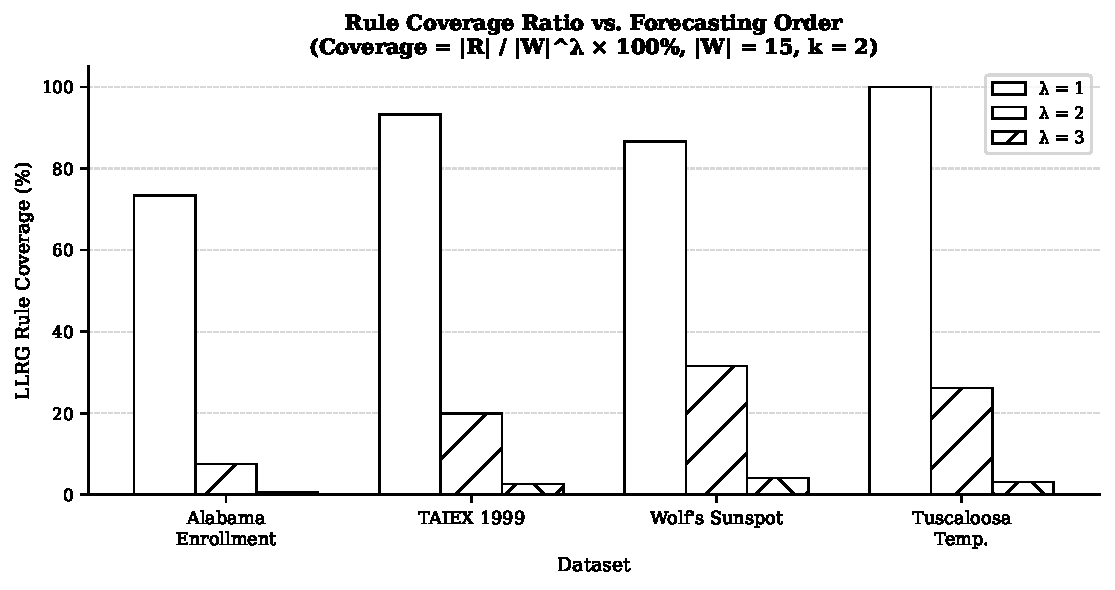
\includegraphics[width=\textwidth]{figures/fig3_coverage.pdf}
  \centerline{\small(a) LLRG Coverage vs.\ Order}
\end{minipage}
\hfill
\begin{minipage}[b]{0.50\textwidth}
  \centering
  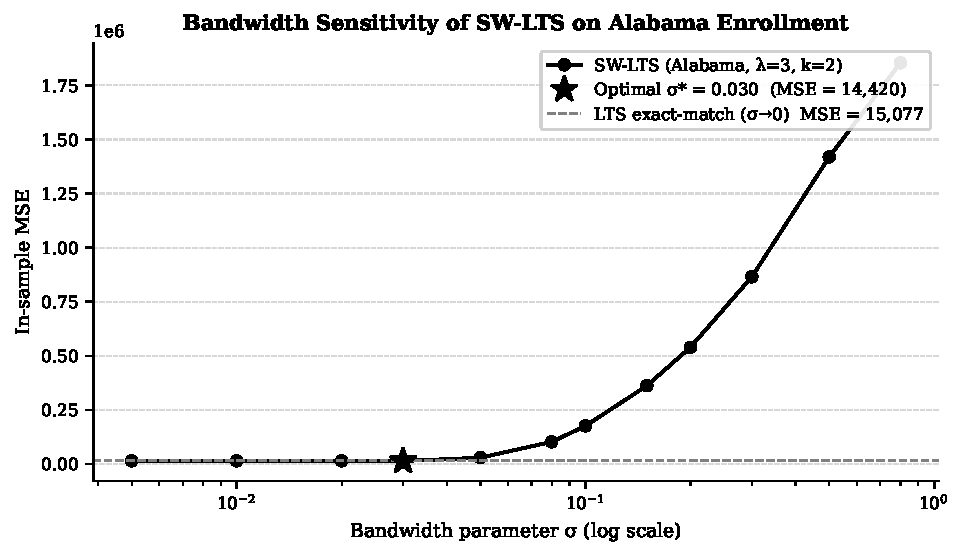
\includegraphics[width=\textwidth]{figures/fig2_sigma_sensitivity.pdf}
  \centerline{\small(b) Bandwidth Sensitivity (Alabama)}
\end{minipage}
\caption{(a) Coverage (\%) at $\lambda=1,2,3$ for all datasets.
(b) MSE vs.\ $\sigma$ on Alabama ($\lambda=3$). Star: in-sample
optimum $\sigma^*{=}0.03$ (MSE~=~14,420); dashed: LTS exact-match
baseline (MSE~=~15,077).}
\label{fig:coverage}
\end{figure}

\subsection{Discussion}
\label{sec:discussion}

\textbf{Sunspot: kernel aggregation over high-dynamic-range cycles.}
Sunspot numbers span 0--296, so HO-LTS's global-mean fallback for
${\approx}96\%$ of unmatched queries is far from the actual value in
both active and quiet solar phases. SW-LTS ($\sigma^*{=}0.020$) kernels
over all 139 training rules, weighting semantically adjacent patterns,
and achieves MSE~=~1,100---below both HO-LTS (3,604, $-$69.5\%,
$p{<}0.001$) and the naive predictor (2,155).

\textbf{Temperature: limits of kernel smoothing.}
On Tuscaloosa Temperature ($23$--$32^{\circ}$C), SW-LTS walk-forward
MSE is 47.7\% higher than HO-LTS (2.145 vs.\ 1.452, $p{=}0.969$),
with both exceeding naive (0.891). The narrow range makes the global
mean a reliable fallback; kernel-weighted rules from phase-shifted
seasons introduce additional error. SW-LTS's benefit requires high
dynamic range with structured periodicity.

\textbf{Interpretability: kernel weight attribution.}
Table~\ref{tab:casestudy} decomposes walk-forward step $t{=}237$
on Sunspot ($y_t{=}190.6$, $\hat{y}_t{=}190.1$, error~0.3\%).
Rule~1 (exact match, Prop.~\ref{prop:sigma0}) takes 99.5\% weight;
Rules~2--3, at HA distance ${\approx}0.07$, share $0.3\%$; all
110 remaining rules together contribute ${<}0.2\%$. This attribution
is impossible under binary lookup and is auditable in the HA
algebraic structure.

\begin{table}[htbp]
\caption{Kernel weight attribution, $t{=}237$, Wolf's Sunspot
($y_t{=}190.6$, $\hat{y}_t{=}190.1$; $\sigma^*{=}0.020$,
$\lambda{=}3$, $M{=}113$). Query: $\bm{\ell}_t{=}(VV^-,LV^-,L^-)$
(${}^-{=}$hedge on $c^-$, Small; e.g., $VV^-{=}V(V(c^-))$).}
\label{tab:casestudy}
\centering\small
\begin{tabular}{@{}c l r r@{}}
\toprule
Rank & LHS $\bm{k}_j$ & $\bar{s}(R_j)$ & $w_j$ \\
\midrule
1 & $(VV^-,\,LV^-,\,L^-)$ & 190.1 & 99.5\% \\
2 & $(VV^-,\,LV^-,\,LL^-)$ & 147.2 & 0.2\% \\
3 & $(V^-,\,LV^-,\,L^-)$ & 199.4 & 0.1\% \\
\midrule
\multicolumn{3}{@{}l}{\small Remaining 110 rules} & ${<}0.2\%$ \\
\bottomrule
\end{tabular}
\end{table}

\textbf{Why LTS-PSO cannot fix sparsity.}
With $n{-}\lambda{=}19$ $\lambda$-grams, the $0.56\%$ ceiling holds
regardless of $(\theta,\alpha)$: the lookup mechanism must change.

% ─────────────────────────────────────────────────────────────────────────────
\section{Conclusion}
\label{sec:conclusion}

SW-LTS advances LTS forecasting on two fronts. \emph{Interpretability}:
graded kernel aggregation makes every prediction a linguistically
auditable weighted average of stored rules, with weights derived from
the HA algebraic structure---demonstrated via kernel weight attribution
at $t{=}237$ on Sunspot (Table~\ref{tab:casestudy}). \emph{Generalization}:
we formally characterize the sparse-rule problem (coverage decays to
0.56\% on Alabama at $\lambda{=}3$) and prove SW-LTS recovers both LTS
($\sigma\to 0$) and HO-LTS ($\sigma\to\infty$). In-sample experiments
confirm SW-LTS matches or improves the best baseline across four
datasets; walk-forward validation shows a significant 69.5\% MSE
reduction on Wolf's Sunspot ($p{<}0.001$). Future work includes adaptive bandwidth, multi-step forecasting,
and non-Gaussian kernels compatible with the HA partial order.

\subsubsection*{Disclosure of Interests}
The author has no competing interests to declare relevant to this
article.

% ─────────────────────────────────────────────────────────────────────────────
\begin{thebibliography}{16}

\bibitem{dixit2023fts}
Dixit, A., Jain, S.: Intuitionistic fuzzy time series forecasting for
non-stationary data with suitable cluster count and window size.
Inf. Sci. \textbf{623}, 132--145 (2023).
\url{https://doi.org/10.1016/j.ins.2022.12.015}

\bibitem{feng2025interp}
Feng, J., Gong, Z.: An interpretable combined forecasting method for
stock market based on fuzzy time series and linear-trend fuzzy
information granulation.
IEEE Access \textbf{13}, 73722--73734 (2025).
\url{https://doi.org/10.1109/ACCESS.2025.3564135}

\bibitem{chen1996}
Chen, S.-M.: Forecasting enrollments based on fuzzy time series.
Fuzzy Sets Syst. \textbf{81}(3), 311--319 (1996).
\url{https://doi.org/10.1016/0165-0114(95)00220-0}

\bibitem{hieu2020lts}
Hieu, N.D., Ho, N.C., Lan, V.N.: Enrollment forecasting based on
linguistic time series. J. Comput. Sci. Cybern. \textbf{36}(2),
119--137 (2020).
\url{https://doi.org/10.15625/1813-9663/36/2/14965}

\bibitem{hieu2021holts}
Hieu, N.D.: Scalable human knowledge about numeric time series
variation and its role in improving forecasting results.
J. Comput. Sci. Cybern. \textbf{38}(2), 97--120 (2022).
\url{https://doi.org/10.15625/1813-9663/38/2/16866}

\bibitem{hieu2022ltspso}
Hieu, N.D., Linh, M.V., Phong, P.D.: Linguistic time series
forecasting based on particle swarm optimization for hedge algebra
parameter tuning. J. Comput. Sci. Cybern. \textbf{38}(4), 317--335
(2022). \url{https://doi.org/10.15625/1813-9663/38/4/17261}

\bibitem{hieu2023colts}
Hieu, N.D., Linh, M.V., Phong, P.D.: A co-optimization algorithm
utilizing particle swarm optimization for linguistic time series.
Mathematics \textbf{11}(7), 1597 (2023).
\url{https://doi.org/10.3390/math11071597}

\bibitem{catho2002ha}
Ho, N.C., Wechler, W.: Hedge algebras: An algebraic approach to
structure of sets of linguistic truth values.
Fuzzy Sets Syst. \textbf{35}(3), 281--293 (1990).
\url{https://doi.org/10.1016/0165-0114(90)90002-U}

\bibitem{catho2002sqm}
Ho, N.C., Long, N.V.: Fuzziness measure on complete hedge algebras
and quantifying semantics of terms in linear hedge algebras.
Fuzzy Sets Syst. \textbf{158}(4), 452--471 (2007).
\url{https://doi.org/10.1016/j.fss.2006.10.023}

\bibitem{kennedy1995pso}
Kennedy, J., Eberhart, R.: Particle swarm optimization.
In: Proc. IEEE Int. Conf. Neural Networks, pp.~1942--1948. IEEE
(1995). \url{https://doi.org/10.1109/ICNN.1995.488968}

\bibitem{koczy1993fri}
K\'{o}czy, L.T., Hirota, K.: Approximate reasoning by linear rule
interpolation and general approximation.
Int. J. Approx. Reason. \textbf{9}(3), 197--225 (1993).
\url{https://doi.org/10.1016/0888-613X(93)90010-B}

\bibitem{nadaraya1964}
Nadaraya, E.A.: On estimating regression.
Theor. Probab. Appl. \textbf{9}(1), 141--142 (1964).
\url{https://doi.org/10.1137/1109020}

\bibitem{song1993}
Song, Q., Chissom, B.S.: Forecasting enrollments with fuzzy time
series---Part~I. Fuzzy Sets Syst. \textbf{54}(1), 1--9 (1993).
\url{https://doi.org/10.1016/0165-0114(93)90355-L}

\bibitem{song1994}
Song, Q., Chissom, B.S.: Forecasting enrollments with fuzzy time
series---Part~II. Fuzzy Sets Syst. \textbf{62}(1), 1--8 (1994).
\url{https://doi.org/10.1016/0165-0114(94)90067-1}

\bibitem{yu2005}
Yu, H.-K.: Weighted fuzzy time series models for TAIEX forecasting.
Phys. A \textbf{349}(3--4), 609--624 (2005).
\url{https://doi.org/10.1016/j.physa.2004.10.032}

\bibitem{zhan2024dfcnn}
Zhan, T., He, Y., Deng, Y., Li, Z.: Differential convolutional fuzzy
time series forecasting. IEEE Trans. Fuzzy Syst. \textbf{32}(2),
294--306 (2024).
\url{https://doi.org/10.1109/TFUZZ.2023.3290489}

\end{thebibliography}

\end{document}
